\documentclass{article}
\usepackage[final]{neurips}
\usepackage[framemethod=tikz]{mdframed}
\usepackage{lipsum}
\definecolor{mycolor}{rgb}{0.122, 0.435, 0.698}
\newmdenv[innerlinewidth=0.5pt, roundcorner=4pt,linecolor=mycolor,innerleftmargin=6pt,
innerrightmargin=6pt,innertopmargin=6pt,innerbottommargin=6pt]{mybox}
\usepackage[utf8]{inputenc} % allow utf-8 input
\usepackage[T1]{fontenc}    % use 8-bit T1 fonts
\usepackage[hidelinks]{hyperref}       % hyperlinks
\usepackage{url}            % simple URL typesetting
\usepackage{booktabs}       % professional-quality tables
\usepackage{amsfonts}       % blackboard math symbols
\usepackage{nicefrac,tcolorbox}       % compact symbols for 1/2, etc.
\usepackage{amsmath}
\usepackage{microtype}      % microtypography
\usepackage{graphicx,caption}
\usepackage{xepersian}
\settextfont{XB Niloofar}
\setdigitfont{XB Niloofar}

\title{
	\vspace{-0.8em}
تمرین سری اول درس نظریه گروه‌ها - دکتر رضاخانی
\\
{\normalsize
\textbf{مهلت تحویل:
شنبه ۱۲ اسفند ماه سال ۱۴۰۲ تا ساعت ۲۳:۵۹ 
\\
\vspace{-0.4em}
از طریق سامانه
\href{https://cw.sharif.edu/}{درس‌افزار شریف}
}
}
\vspace{-0.6em}
}

\usepackage[utf8]{inputenc}

\usepackage[english]{babel}
\setlength{\parindent}{3.5em}
\setlength{\parskip}{0.5em}
\renewcommand{\baselinestretch}{1.0}

\usepackage{calrsfs}
\DeclareMathAlphabet{\pazocal}{OMS}{zplm}{m}{n}
\newcommand{\La}{\mathcal{L}}
\newcommand{\Lb}{\pazocal{L}}

\newtcolorbox{boxes}[3][]
{
	colframe = #2!25,
	colback  = #2!10,
	coltitle = #2!40!black,  
	title    = {\textbf{#3}},
	#1,
}

\newenvironment{exercise}[3][\unskip]{%
	\par
	\noindent
	\textbf{تمرین
		#1
		[#2 امتیاز] 
		\def\temp{#3}\ifx\temp\empty
		: 
		\else
		: #3 \vspace{0.5em} \\ \noindent
		\fi
}}{}

\author{
حسین محمدی\\
  \lr{
  		\href{mailto:hossein.mohammadi.00427@gmail.com}{\texttt{	hossein.mohammadi.00427@gmail.com}}} \\
  \And
  زهرا کبیری\\
 \lr{
  		\href{mailto:kabiri.zahra98@gmail.com}{ \texttt{kabiri.zahra98@gmail.com}}}\\
  }

\begin{document}


\begin{minipage}{0.1\textwidth}% adapt widths of minipages to your needs
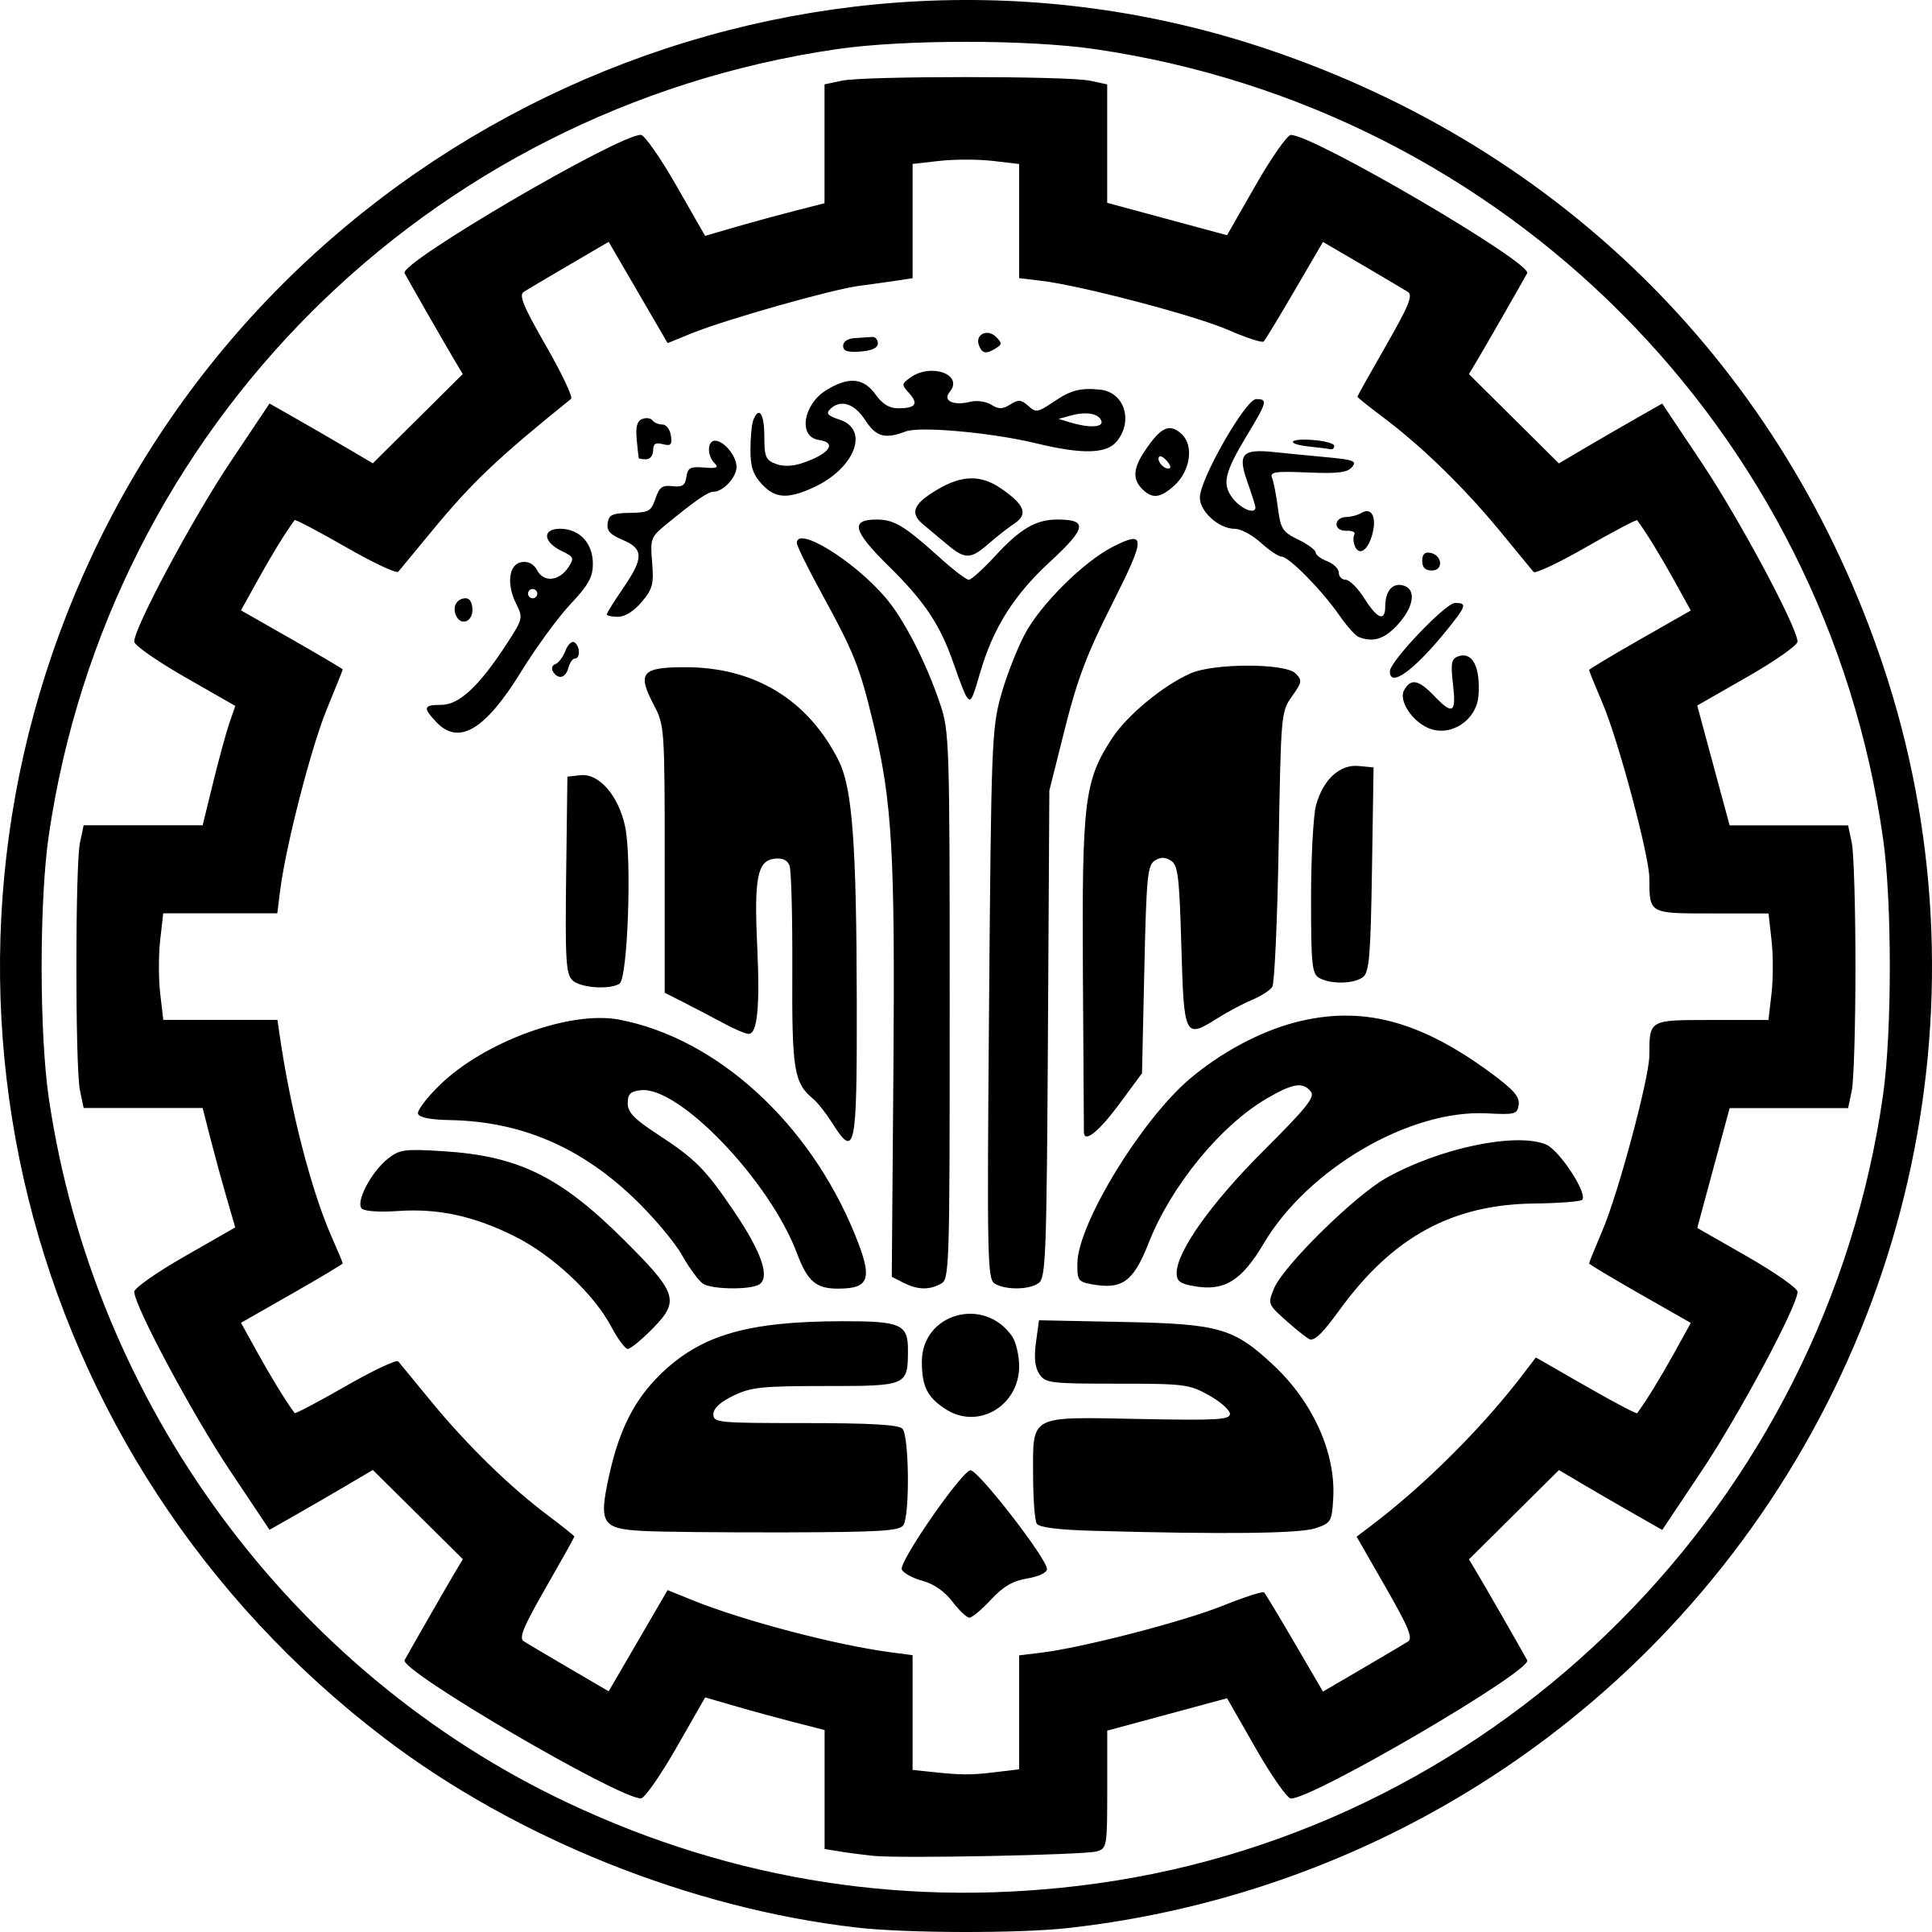
\includegraphics[width=1.1cm]{sharif-logo.png}
\end{minipage}%
\hfill%
\begin{minipage}{0.9\textwidth}\raggedleft
دانشگاه صنعتی شریف\\
زمستان ۱۴۰۲ - بهار ۱۴۰۳\\
\end{minipage}

\makepertitle


%%%%%%%%%%%%%%%%%%%%%%%%%%%%%%%%%%%%%%%%%%%%%%%%%%%%%%%%%%%%%%%%%%
% Write Exerciese Here:



\begin{exercise}[۱]{۱۵}{}
	مجموعه‌ی 
	$G$ 
	را متشکل از زوج‌مرتب‌های حقیقی 
	$(a,b)$
	در نظر بگیرید که 
	$a\neq 0$
.
نشان دهید که با عمل دوتایی زیر، این مجموعه تشکیل یک گروه می‌دهد.
\[
. : G \times G \to  G \;\;\;\;\;\;:\;\;\;\;\;\;\;\;
(a,b).(c,d) = (ac,ad+b)
\]
\end{exercise}



\begin{exercise}[۲]{۲۰}{\href{https://en.wikipedia.org/wiki/Central_subgroup}{زیرگروه مرکزی}}
 زیرگروه مرکزی یک گروه 
 $G$
 ، 
 مجموعه‌ی اعضائی از 
 $G$
 است که با تمامی اعضای گروه $G$ جابه‌جا می‌شوند.
 \[
 Z(G) = \{z\in G | zg = gz \;, \; \forall g\in G\}
 \]
 نشان دهید  که 
 $Z(G)$
 با عمل ضرب روی $G$ خود تشکیل یک گروه جابه‌جایی می‌دهد
 \LTRfootnote{Abelian subgroup}
 .
 \begin{boxes}{black}{تعریف گروه آبلی یا گروه جابه‌جایی:}
 	عمل‌دوتایی روی گروه \textbf{لازم}‌ است که خاصیت انجمنی
 	\LTRfootnote{Associative}
 	داشته باشد، یعنی برای هر سه عضو 
 	$g_1 , g_2 , g_3 \in G$
 	داشته باشیم:
 	\[
 	g_1.(g_2.g_3) = (g_1.g_2).g_3
 	\]
 	اگر علاوه بر‌این، خاصیت جابه‌جایی هم داشته باشد؛ یعنی برای هر دو عضو 
 	$g_1 , g_2  \in G$
 	داشته باشیم
 	\[g_1.g_2 = g_2.g_1\]
 	آنگاه این گروه، گروه جابه‌جایی یا گروه آبلی نامیده می‌شوند.
 	
 	فکرکنید که آیا تعریف جابه‌جایی و تعریف انجمنی کاملا از هم مستقل اند؟ آیا می‌توانید عملی دوتایی تعریف کنید که جابه‌جایی باشد اما انجمنی نباشد؟
 	 
 \end{boxes} 
 
\end{exercise}

\begin{exercise}[۳]{15}{}
	 نشان دهید که اگر در یک گروه، هرعضو وارون خودش باشد، آن گروه حتما جابه‌جایی است.
\end{exercise}




\vspace{2em}
\begin{exercise}[۴]{۳۵}{}
	فرض کنید 
	$S$
	یک مجموعه با عمل دوتایی شرکت‌پذیر باشد و دو شرط زیر در آن برقرار باشند:
	\begin{enumerate}
		\item عنصر 
		$e\in S$ 
		موجود باشد به طوری که برای هر 
		$s \in S$
		داشته باشیم 
		$s = se$\footnote{با تشکر از آقای آرشا نیک‌سا.}.
		\item برای هر 
		$s\in S$
		عنصر 
		$ s^{'}$
		موجود باشد به طوری که 
		$s s^{'} = e$.
	\end{enumerate}
	نشان دهید که 
	$e$
	عضو خنثای 
	$S$
	است و هر عضو 
	$S$
	وارون‌پذیر است.
\end{exercise}

\begin{exercise}[۵]{۱۵}{
	گروه چندوجهی 
	$D_5$
	}
	گروه 
	$D_5$
	که گروه تقارنی پنج‌وجهی منتظم است، متشکل از دوران هایی با زاویه‌ی ۷۲ درجه نسبت به مرکز، و بازتاب نسبت به محورهای تقارن است؛ در شکل زیر عمل اعضای گروه را روی پنج وجهی می‌بینید.
	\begin{figure}
		\centering
		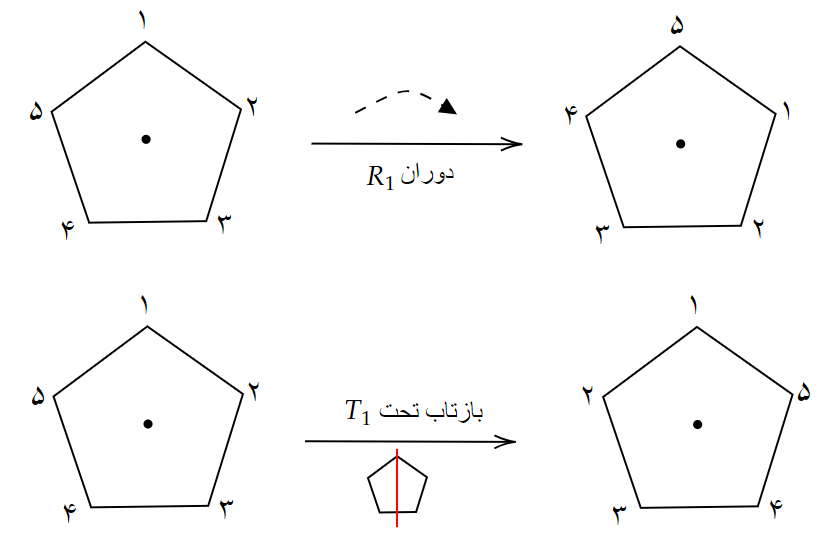
\includegraphics[width=35em]{1.png}
		\captionsetup{labelformat=empty}
		\caption{تصویر ۱: اثر گروه 
		$D_5$
		روی پنج وجهی منتظم.
		}
		\label{fig1}
	\end{figure}
	پس این گروه حداقل ۱۰ عضو دارد (هنوز مطمئن نیستیم که حاصل ضرب اعضا بسته باشد.)
	
	\noindent
	دوران‌ها را $R_i$ و بازتابها را $T_i$ بنامید و جدول ضرب اعضای این مجموعه را بنویسید. یعنی جدولی مانند شکل 
	\ref*{fig2}
	 درست کنید و تک‌‌‌تک حاصل‌ضرب‌ها را در آن وارد کنید.
	
	\begin{figure}[h]
		\centering
		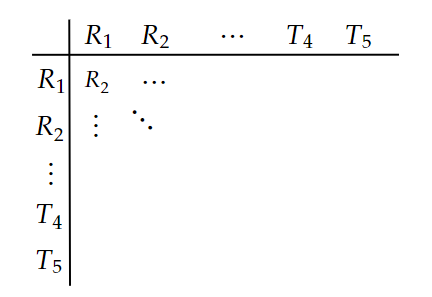
\includegraphics[width=20em]{2.png}
		\captionsetup{labelformat=empty}
		\caption{تصویر ۲: جدول‌ضرب گروه 
			$D_5$.
		}
		\label{fig2}
	\end{figure}
	\noindent
	آیا نیاز هست که عضوی اضافه شود تا مجموعه تحت عمل ضرب بسته باشد و تشکیل یک گروه بدهد؟ آیا گروه حاصل جابه‌جایی است؟ مرتبه‌ی هریک از اعضا را بنویسید.
	
	 \begin{boxes}{black}{مرتبه‌ی یک عضو از گروه:}
	مقصود از مرتبه‌ی یک عضو $a\in G$، کوچکترین عددی طبیعی $N$ است که 
	$\underbrace{a\times a\times \dots \times a}_{\text{\lr{N} بار}} = e$ 
	که در آن $e$ عضو خنثی گروه است .
	
	\noindent
	مثلا در گروه 
	$\mathbb{Z}_5$
	که متشکل از اعداد 
	$\{0,1,2,3 , 4\}$
	با عمل جمع به پیمانه‌ی $5$ است؛ مرتبه‌ی تمامی اعضا (به غیر صفر) پنج است.
	گاهی مرتبه تعریف نمی‌شود؛ مثلا در گروه اعداد صحیح با عمل جمع، مرتبه تعریف نمی‌شود چرا که حاصل جمع هر عدد غیر صفر با خودش، هرگز صفر نمی‌شود.
		
	\end{boxes} 
\end{exercise}


 \end{document}
